\part{Basic texture mapping}
\frame{\partpage}

\begin{frame}{Loading textures from a file}
	\begin{itemize}
		\item The \textbf{SDL\_Image library} lets us load images from JPG, PNG, BMP etc.
		\pause\item Steps:
			\begin{itemize}
				\pause\item Load the image with \lstinline{IMG_Load}
				\pause\item Create a texture with \lstinline{glGenTextures}
				\pause\item Bind the texture with \lstinline{glBindTexture}
				\pause\item Load the pixel data into the new texture with \lstinline{glTexImage2D}
				\pause\item Set the texture filtering modes with \lstinline{glTexParameteri} (more on this later)
			\end{itemize}
	\end{itemize}
\end{frame}

\begin{frame}{Texture coordinates}
	\begin{itemize}
		\item We use \textbf{UV coordinates} to refer to points in a texture
		\pause\item $u$ axis is horizontal and ranges from 0 (left) to 1 (right)
		\pause\item $v$ axis is vertical and ranges from 0 (bottom) to 1 (top)
		\pause\item (So really just another name for $xy$ coordinates in texture space)
		\pause\item Basic idea of texture mapping: give each vertex a $uv$ coordinate, and interpolate across the triangle
	\end{itemize}
\end{frame}

\begin{frame}{UV coordinates}
	\begin{center}
		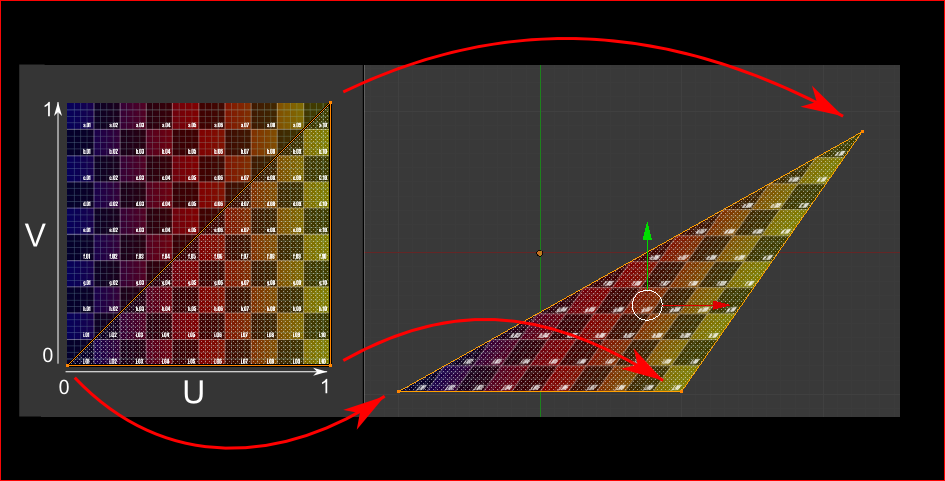
\includegraphics[width=\textwidth]{uv}
	\end{center}
\end{frame}

\fullbleed{character_texture}

\begin{frame}[fragile]{Textures in GLSL}
	Fragment shader:
	
	\begin{lstlisting}[language=GLSL]
in vec2 textureCoords;
uniform sampler2D textureSampler;

void main()
{
    fragmentColour = texture(textureSampler, textureCoords);
}
	\end{lstlisting}
\end{frame}

\begin{frame}[fragile]{Texture filtering}
	\pause
	\begin{lstlisting}
glTexParameteri(GL_TEXTURE_2D, GL_TEXTURE_MIN_FILTER, GL_LINEAR);
glTexParameteri(GL_TEXTURE_2D, GL_TEXTURE_MAG_FILTER, GL_LINEAR);
	\end{lstlisting}
	\begin{itemize}
		\item \textbf{Linear interpolation} (\lstinline{GL_LINEAR})
			smooths between pixels
		\pause\item \textbf{Nearest neighbour} (\lstinline{GL_NEAREST})
			is pixelated but may be slightly faster
		\pause\item \textbf{Anisotropic filtering} improves the quality of linear interpolation
			but is slower
		\pause\item \textbf{Mip-mapping} pre-calculates scaled down versions of the texture ---
			improves quality but costs memory
	\end{itemize}
\end{frame}

\begin{frame}{Texture dimensions}
	\begin{itemize}
		\item In the old days, OpenGL required textures to have \textbf{power of two} dimensions
			\begin{itemize}
				\pause\item $2, 4, 8, 16, 32, 64, 128, 256, 512, 1024, \dots$
			\end{itemize}
		\pause\item Nowadays \textbf{non-power of two (NPOT)} textures are widely supported
		\pause\item Still better to stick to powers of two as some things work better (e.g.\ mipmapping)
		\pause\item NB: \textbf{rectangular} textures are fine, but \textbf{square} textures make UV coordinates saner
	\end{itemize}
\end{frame}

\begin{frame}
	\begin{center}
		Texture Mapping Example
	\end{center}
\end{frame}
